\documentclass{beamer} % "Beamer" is a word used in Germany to mean video projector. 

\usetheme{Berlin} % Search online for beamer themes to find your favorite or use the Berkeley theme as in this file.
\usepackage[slovene]{babel}
\usepackage[cp1250]{inputenc}
\usepackage{color} % It may be necessary to set PCTeX or whatever program you are using to output a .pdf instead of a .dvi file in order to see color on your screen.
\usepackage{graphicx} % This package is needed if you wish to include external image files.

\usepackage{amsmath,amssymb,amsfonts}
\usepackage{url}
\usepackage{authblk}

%\theoremstyle{definition} % See Lesson Three of the LaTeX Manual for more on this kind of "proclamation."
%\newtheorem*{dfn}{A Reasonable Definition}               

\title{Skriti markovski modeli v finančnih časovnih vrstah}
%\newcommand{\imeavtorja}{Martin Praček} % ime avtorja
%\newcommand{\imementorja}{izr. prof. dr. Damjan Škulj}
\institute{Fakulteta za matematiko in fiziko, Univerza v Ljubljani}
%\date{January 6, 2012} 
% Remove the % from the previous line and change the date if you want a particular date to be displayed; otherwise, today's date is displayed by default.

%\AtBeginSection[]  % The commands within the following {} will be executed at the start of each section.
%{%
%\begin{frame} % Within each "frame" there will be one or more "slides."  
%\frametitle{} % This is the title of the outline.
%\tableofcontents[currentsection]  % This will display the table of contents and highlight the current section.
%\end{frame}
%} % Do not include the preceding set of commands if you prefer not to have a recurring outline displayed during your presentation.

\begin{document}
\begin{frame}
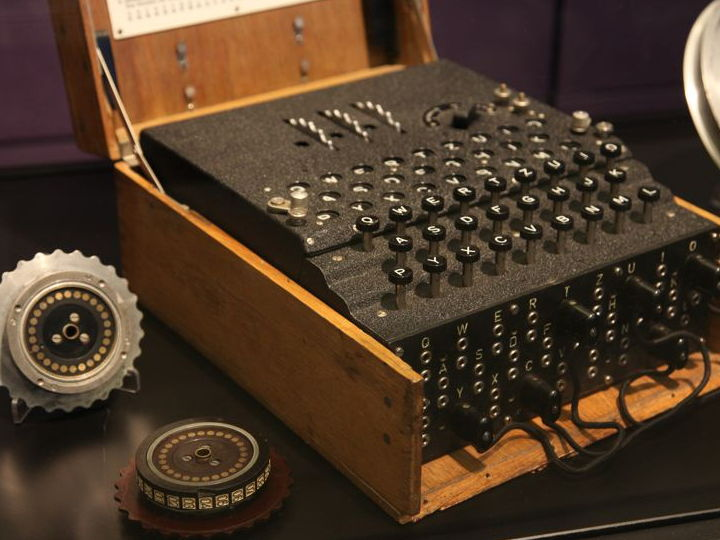
\includegraphics[width=.3\linewidth]{slike/enigma}\quad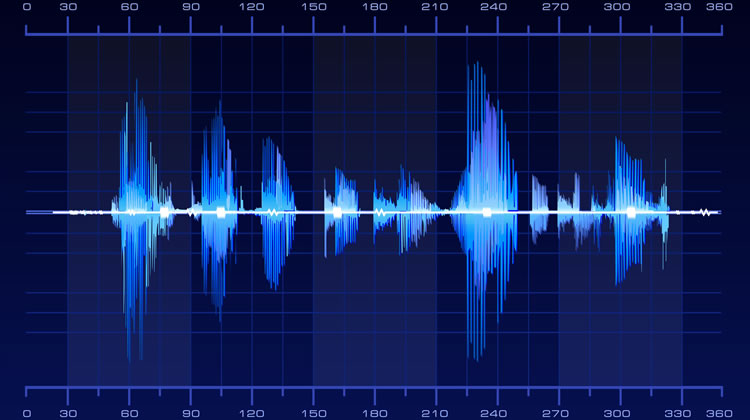
\includegraphics[width=.3\linewidth]{slike/govor}\quad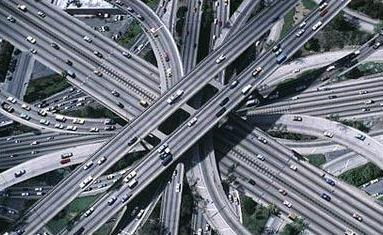
\includegraphics[width=.3\linewidth]{slike/transport}
\\[\baselineskip]% adds vertical line spacing

\includegraphics[width=.3\linewidth]{slike/lastnorocna}\quad
\includegraphics[width=.3\linewidth]{slike/gen}\quad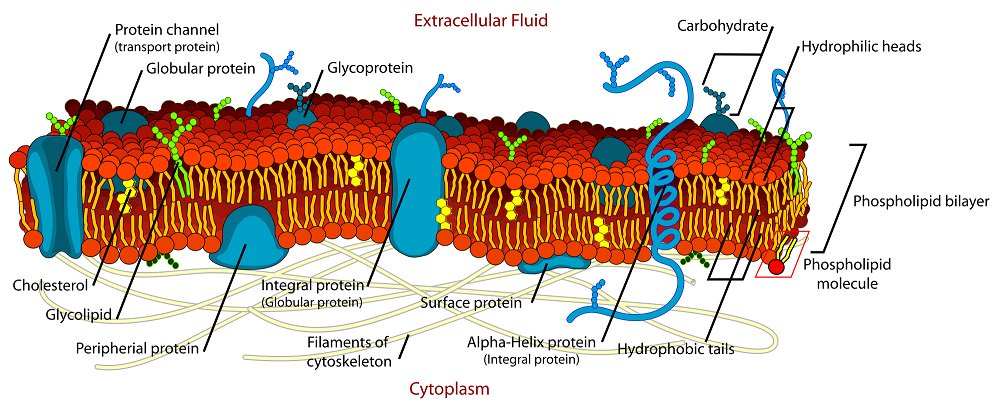
\includegraphics[width=.3\linewidth]{slike/celica1}
\end{frame}	

\begin{frame} 
\begin{titlepage}
	\begin{center}
		\vspace*{1cm}
		Martin Praček \\
		Mentor: izr. prof. dr. Damjan Škulj
		
		\vspace{3cm}
		
\includegraphics[scale=1]{slike/logo}
		
		
		\vfill
		
		\large Ljubljana, december 2018
		
	\end{center}
\end{titlepage}
\end{frame}

%\section{Markovski model} % Since this is the start of a new section, our recurring outline will appear here.

\begin{frame} 
\frametitle{Markovski model}
\begin{itemize}
	\item Markovska lastnost je lastnost slučajnega procesa v diksretnem času, da je njegova vrednost v času $t$ odvisna le od njegove vrednosti v času $t-1$.
	\item Ločimo v celoti opazovan in delno opazovan ter
	\item Avtonomen in kotroliran sistem.
\end{itemize}
\includegraphics[scale=0.5]{slike/veriga}
\end{frame}


\begin{frame}
\frametitle{Delitev markovskih modelov}
\includegraphics[width=10cm]{slike/slika1.png}
\end{frame}

%\section{Skriti markovski model}
\begin{frame}
\frametitle{Skriti markovski model}
Skriti markovski model je statistični markovski model, kjer predpostavljamo, da je modelirani sistem markovski proces z skritimi stanji.\\
Gre torej za tip modela, kjer lahko razberemo rezultat, ne moremo pa ugotoviti, kakšna je bila funkcija, ki nam ga je dala. 
\includegraphics[scale=0.25]{slike/hmm2} 
\end{frame}

\begin{frame}
\frametitle{Zahteve}
\begin{itemize}
	\item Markovska lastnost
	\item Enakomerno porazdeljeni časi signalov $O_{t}$, ki jih poda resnični svet
	\item Sistem ima $N$ stanj, vsako določa slučajna spremenjivka $S$
\end{itemize}
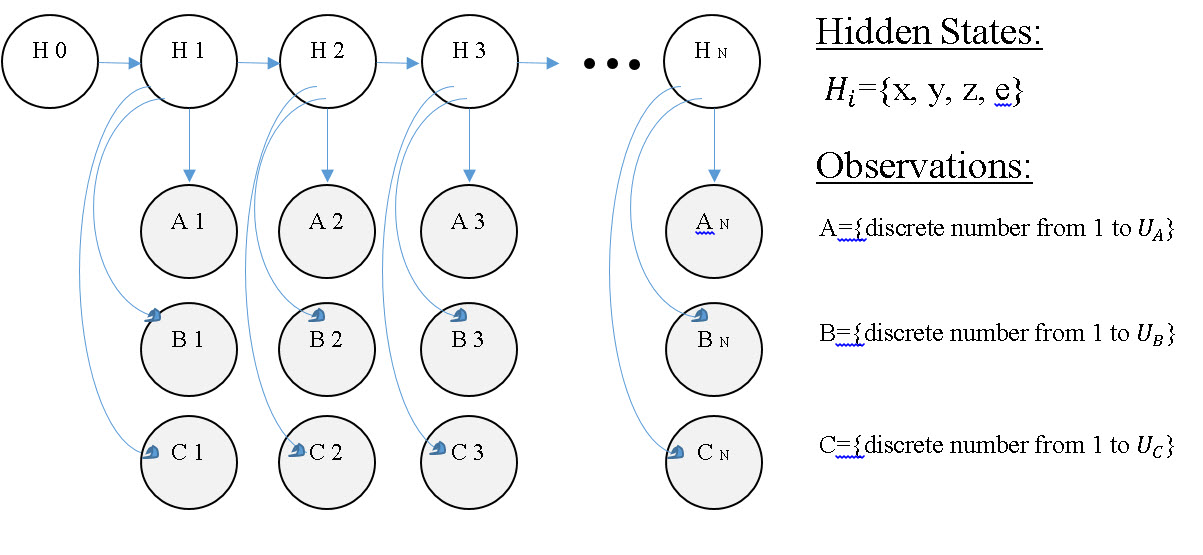
\includegraphics[scale=0.25]{slike/hmm}
\end{frame}

\begin{frame}
\begin{itemize}
	\item Slučajnih spremenljivk skritih skoraj v nobenem času ne poznamo, poznamo pa slučajni proces $Q$, ki predstavlja signale
	\item Porazdelitveni zakon vsakega stanja $i$ označimo z $b_{i}(x)$
	\item Vektor začetnih stanj je $\pi$
	\item Prehodna matrika $A$, ki je neodvisna od časa
\end{itemize}
\end{frame}

\begin{frame}
\frametitle{Porazdelitveni zakon}
\begin{itemize}
	\item Gaussova mešanica
	\item  $b_{i} = \sum_{j = 1}^{M}{c_{ij}} N(x;\mu_{j}, \sigma_{j}^2)$
	\item Število porazdelitev $M$
	\item Matrika $\Gamma$, $\mu_{ij}$ predstavlja pričakovano vrednost porazdelitve $j$ v stanju $i$
	\item Matrika $\Sigma$, kjer $\sigma_{ij}$ predstavlja varianco porazdelitve $j$ v stanju $i$
	\item Matrika $C$, koeficienti $c_{ij}$ iz Gaussove mešanice
\end{itemize}
\end{frame}

\begin{frame}
\frametitle{Osnovanje modela}
Da bomo lahko delali z našim modelom, moramo najprej izvesti t.i. trening modela.
\begin{itemize}
	\item Razvrščanje v skupine ($k$-means clustering)
	\item Akaikov informacijski kriterij
\end{itemize}
\includegraphics[scale=0.35]{slike/delnica}
\end{frame}

\begin{frame}
\frametitle{Izračun  $P(O|\lambda)$}
Z $\lambda$ označimo vse ostale parametre  $\lambda$ $=$ $(\pi,A,C,\Gamma,\Sigma)$.
Za učinkovit izračun le teh si pomagamo z iterativnim postopkom, podobnim sistemu EM, $naprej - nazaj$.
$$\alpha_{1}(i) = \pi_{i}b_{i}(O_{1}) = \pi_{i}b_{i} = \sum_{k = 1}^{M}{c_{ik}}$$
$$\Downarrow$$
$$P(O|\lambda) = \sum_{i=1}^{N}{\alpha_{T}(i)}$$
\end{frame}

\begin{frame}
\frametitle{Trening modela}
Da bomo lahko $P(O|\lambda)$ maksimizirali, potrebujemo začetne ocene parametrov. 
Za to ne poznamo analitičnega postopka, lahko pa lokalno maksimiziramo, z naprimer, Baum-Welchovim algoritmom.
Pri tem nas ne skrbijo ocene za $A$ ter $\pi$, kjer moramo paziti le na neničelnost le teh.
Več problemov nam povzročajo  $C$, $\Sigma$ in $\Gamma$.
\end{frame}

\begin{frame}
\frametitle{ $C$, $\Sigma$ in $\Gamma$}
 Za dobro začetno oceno si lahko pomagamo z razvrščanjem v skupine.
 Za $C$ to pomeni, da bo element $c_{ij}$ $=$ $1/M$ za vsak par $ij$, kjer je $M$ število skupin. Pričakovane vrednosti in variance nato pridobimo iz vrednosti teh skupin.
 \ \\
 \includegraphics[scale=0.5]{slike/kmeans}
\end{frame}

\begin{frame}
\frametitle{Lokalno maksimiziranje}
Za potrebe lokalne maksimizacije določimo dodatne funkcije:
$$\xi_{t}(i,j) = \frac{\alpha_{t}(i)a_{ij}b_{j}(O_{t})\beta_{t+1}(j)}{P(O|\lambda)}$$
$$\gamma_{t}(i) = \frac{\alpha_{t}(i)\beta_{t}(i)}{P(O|\lambda)}$$
$$ \gamma_{t}(j,k) =\gamma_{t}(j)\frac{c_{jk} N(x;\mu_{jk}, \sigma_{jk}^2)}{\sum_{m = 1}^{M}{c_{jm}} N(x;\mu_{jm}, \sigma_{jm}^2)}$$
\begin{center}
	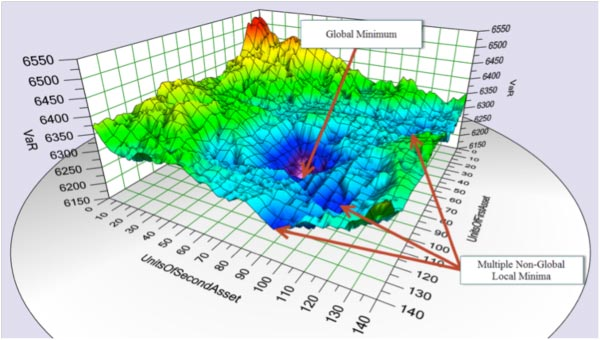
\includegraphics[scale=0.25]{slike/gore}
\end{center}
\end{frame}

\begin{frame}
\frametitle{Lokalno maksimiziranje}
Prek dodatnih funkcij definiramo iteracijske postopke za naše spremenljivke:
$$ \overline{\pi_{i}} = \gamma_{1}(i)$$
$$ \overline{a_{ij}} = \frac{\sum_{t=1}^{T-1}{\xi_{t}}}{\sum_{t=1}^{T-1}{\gamma_{t}(i)}}$$
$$\overline{c_{jk}}= \frac{\sum_{t=1}^{T}{\gamma_{t}(j,k)}}{\sum_{t=1}^{T}\sum_{m=1}^{M}{\gamma_{t}(j,m)}}$$
$$\overline{\mu_{jk}}=\frac{\sum_{t=1}^{T}{\gamma_{t}(j,k)}O_{t}}{\sum_{t=1}^{T}{\gamma_{t}(j,k)}}$$
Tako definiramo večfazni iterativni proces, pri katerem popravljamo vrednosti parametrov do konvergence.
\end{frame}
\begin{frame}
\frametitle{Začetno stanje in Viterbijev algoritem}
Za delo s tem algoritmom moramo definirati $\delta_{t}(i)$, ki za vsako stanje $i$ vrne največjo verjetnost vzdolž poti v času $t$. Prek $\delta_{t}(i)$ nato induktivno izvedemo algoritem.\\
Viterbijev algoritem nam vrne $p*$, ki je največja verjetnost in $q_{T}*$, ki nam pove stanje v času $T$, ki nam to verjetnost vrne.
\end{frame}

\begin{frame}
\frametitle{Uporaba}
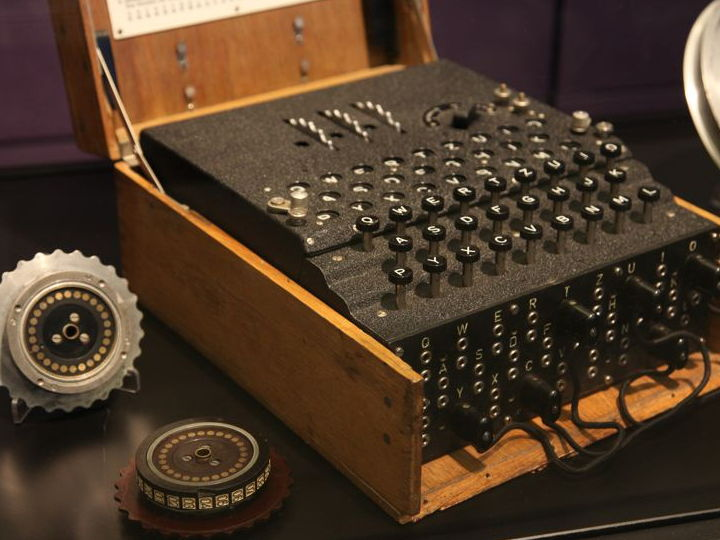
\includegraphics[width=.3\linewidth]{slike/enigma}\quad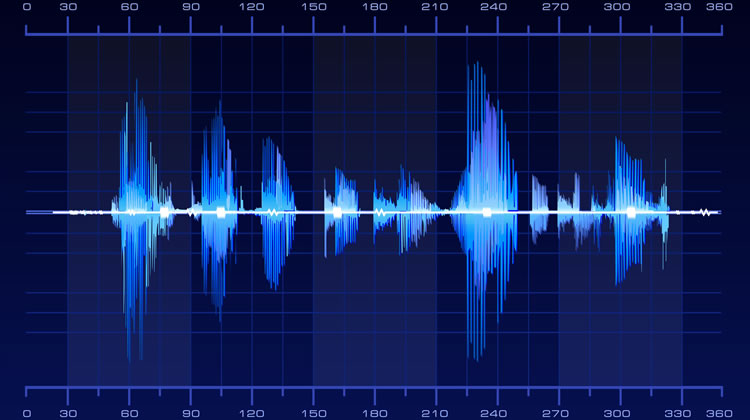
\includegraphics[width=.3\linewidth]{slike/govor}\quad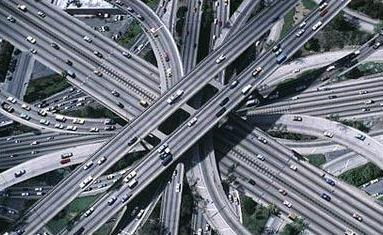
\includegraphics[width=.3\linewidth]{slike/transport}
\\[\baselineskip]% adds vertical line spacing

\includegraphics[width=.3\linewidth]{slike/lastnorocna}\quad
\includegraphics[width=.3\linewidth]{slike/gen}\quad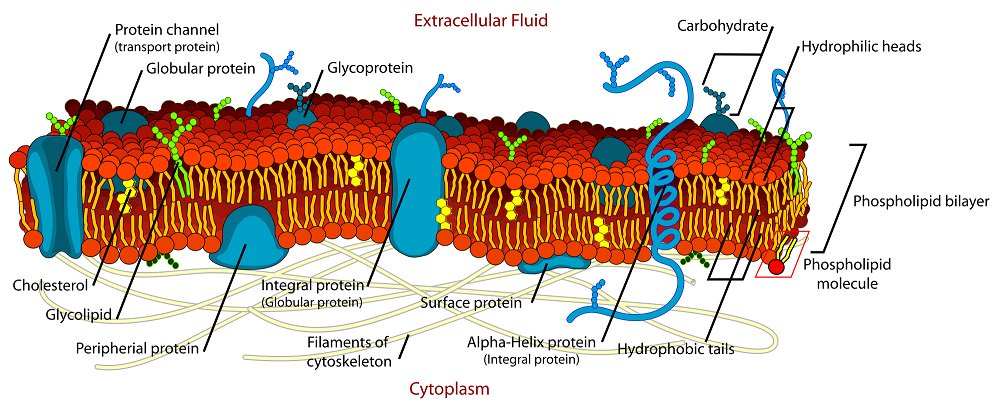
\includegraphics[width=.3\linewidth]{slike/celica1}
\end{frame}	


\begin{frame}
V dolgi predstavitvi se bom bolj posvetil sami finančni analizi, ki sem jo tokrat zaenkrat pustil pri miru.
V prihodnje bom tudi sam poizkusil določiti skriti markovski model na svojem setu podatkov.

\end{frame}

\begin{frame}
\frametitle{Viri}
\begin{enumerate}
	\item I. MacDonald, W. Zucchini. Hidden Markov and Other Models for Discrete-valued Time Series. Chapman \& Hall/CRC Monographs on Statistics \& Applied Probability. Taylor \& Francis. (1997)
	\item D.Roman, G. Mitra,N. Spagnolo. Hidden Markov models for financial optimization problems.IMA Journal of Management Mathematics. 21 (2010).
	 
\end{enumerate}
\end{frame}


\end{document}

